\documentclass[12pt, a4paper]{report}
\usepackage{lipsum}  
\usepackage{url}
\usepackage{hyperref} 
\usepackage{float}
\usepackage{graphicx}
\graphicspath{{figures/}}

\pagenumbering{arabic}
\title{Bipedal Walking - Reinforcement Learning}
\author{Roberto Figueiredo}
\date{April 2022}


\begin{document}
\begin{titlepage}
    \maketitle 
    \thispagestyle{empty}
\end{titlepage}


\begin{abstract}
 
    This report covers the attempt to develop a bipedal walking pattern using reinforcement learning. 
 
    This project developed a series of experiments progressing from a testing ground using the CartPole environment to a 2D walker and implementation of OpenAI Gym on the RoboCup Team, Bold Hearts, ROS2 environment enabling training for any reinforcement learning task.
    The experiments cover the testing of two different learning implementations and hyperparameter tuning.
    
    
    Although the objective of walking could not be achieved in the target time frame with the limited resources available, the documentation covers the problems found along with how this difficulties were overcome. The implementation chapter will cover how each of the stages was developed, with coding examples for each of the main components.
   
    The results and findings of the experiment will be explored and an attempt to understand what could be changed to achieve achieving the desired outcome.

\end{abstract} 

\section*{Acknowledgement}
\lipsum[1-1]


\pagebreak
\tableofcontents
\pagebreak

\chapter{Introduction}
In this chapter the target problem will firstly be introduced, as will a proposed solution to solve it. To understand the problem, 
background information will be covered to better understand the problem and what it is meant to target.
% can I extend this?

\chapter{Introduction}
 RoboCup is a worldwide competition introduced to bridge the gap between robotics and new advancements in AI technology. Each year thousands of RoboCupers get together to compete and share knowledge and advances in robotics. The Bold Hearts team competes in the RoboCup Soccer Humanoid League, hence the relevance of the problem of  walking for bipedal robots. In this Chapter, these topics will be introduced to understand the problem at study better.

 \section{RoboCup}
 RoboCup is an attempt to advance the field of robotics by providing a common problem and an environment for sharing knowledge and collaboration.
 The Objective of RoboCup is to achieve fully autonomous soccer-playing robots that are able to defeat the FIFA World Cup champions by 2050. 

 RoboCup has since evolved from just soccer and now includes multiple fields, Rescue, Soccer, @Home, Industrial and Junior.
 \cite{RoboCup}

 \section{Soccer League}
 RoboCup Soccer is split into multiple leagues, each with different challenges and focuses. The Small Size league uses small wheeled robots, 
 each team is composed of six robots and play using an orange golf ball while tracked by a top-view camera;
 This enables the robots to abstract from challenges such as complex vision detection, 
 walking and others, enabling the teams to focus on strategy and multi-robot/agent cooperation and 
 control in a highly dynamic environment with a hybrid centralized/distributed system. 

 The middle size League assimilates to the small-size league, but in this case, the robots are of a larger size and must have all sensors on board; 
 The league's primary focus is on mechatronics design, control, and multi-agent cooperation at plan and perception levels.

 RoboCup also has simulation for most of its leagues, allowing the teams to focus on software and avoid the difficulties originated by using real robots hardware.

 The Standard Platform is a step-up from the simulation league as while it uses real robots, NAOs, it allows the teams to focus mainly on software while using real robots and the challenges of using real robots without having to develop custom hardware. Each robot is fully autonomous and takes its own decisions.

 The Humanoid League is the most similar to humans, using robots who mimics its shape. Unlike robots outside the Humanoid League, the task of perception and world modelling is not simplified by using non-human like range sensors, making this the most transversal league, requiring hardware and software development. 
 In addition to soccer competitions, technical challenges take place. 
 Dynamic walking, running and kicking the ball while maintaining balance, visual perception of the ball, other players and the field, self-localization, and team play are among the many research issues investigated in the Humanoid League.
 % TODO: add links to pages and explain the difference between humanoid sizes 

 \section{Bold Hearts, UH RoboCup Team}
 The Bold Hearts are the RoboCup team from the University of Hertfordshire. The team researches and develops software and hardware in the Humanoid League, specifically in the teen size league.
 The robots used by the team are based on the Darwin-OP but incrementally developed using custom 3D printed parts and a new computing unit, Odroid-XU4 and camera, the Logitech C920 Pro. 
 The Robots use ROS2 as an operating system.
 \cite{boldhearts}
 \begin{figure}[H]
 \centering
 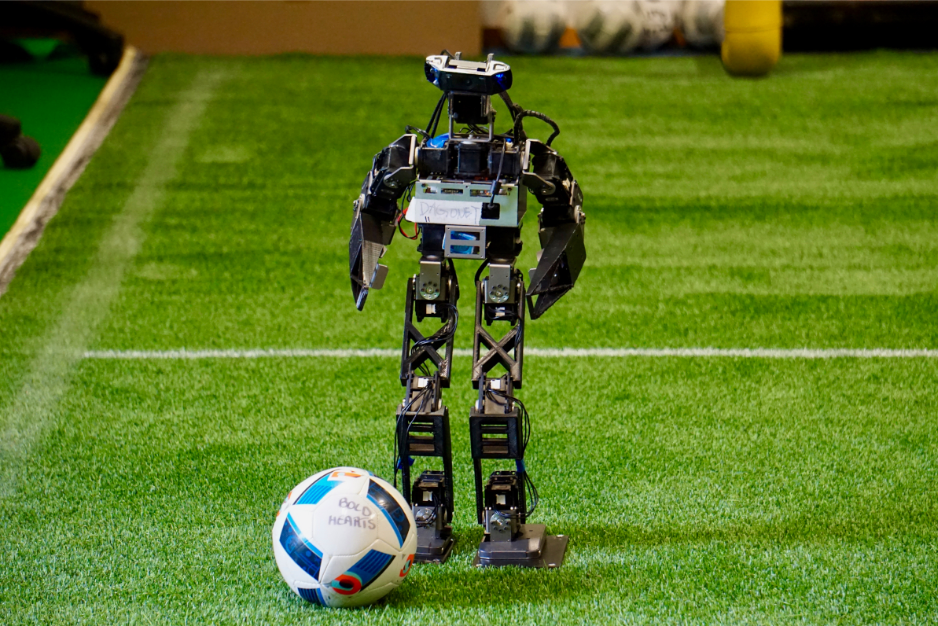
\includegraphics[scale=0.26]{figures/boldbot_2.png}
 \caption{Boldbot, the robot built and used by the Bold Hearts team}
 \end{figure}

 \section{Introduction to the Project}

 \subsection{Problem, Walking for Humanoid robots}
 Until a few years ago, Robotic locomotion was focused on wheel-based movement. Although it is very stable and easy to implement, it lacks flexibility, the ability to move on uneven, unpredictable terrain and overcome obstacles such as stairs.

 The Bold Hearts teams robots must be able to walk and, in addition to the high complexity of this challenge, RoboCup rules periodically change. 
 These changes are implemented as the RoboCup objective is to achieve the most realistic environment and affect both robots, changing the required height, sensors and others, as well as affecting the environment, 
 such as moving from flat ground to synthetic grass. Walking is one of the most complex movements performed by humans, requiring simultaneous control of multiple joints to move while maintaining balance. 
 Not only due to its natural complexity but also aggravated by the rules changes and continuous improvements leading to new updates to the walking algorithm, this is one of the teams most energy and time-consuming problems.
 \subsection{Proposed Solution}

 Walking algorithms can be developed using various techniques, 
 including explicit programming, supervised learning and unsupervised learning. 
 Walking is very complex as there are a lot of variables involved in it, such as the ground contact, 
 maintaining balance and the complex gait movement. The two main aspects important to highlight are that the walking algorithm requires changes when both the robot or external factors change and that it requires manual work from the team to achieve this. 

 The best way to solve the first mentioned problem requires having a robot and environment agnostic approach. This is possible by using reinforcement learning as the principles of the movement maintain, therefore, it should be possible to develop an agnostic reward function.
 From the moment a reinforcement learning solution is successfully implemented, the team should be able to use the same implementation to retrain the policy using the updated robot/environment modelled in the simulator.
 This also reduces the complexity of the problem as the input into the system is sensory data, and the output is a set of actions to execute on the joints.

 \subsection{Aims and Objectives}
 This project proposes to develop a reinforcement learning implementation for walking, 
 to achieve the objectives of the project, three main topics will be covered, 
 robotics biped locomotion, reinforcement learning algorithms and the training framework.

 This project aims to develop an implementation of reinforcement learning to achieve a walking pattern for humanoid robots. 
 It aims to develop detailed documentation on the processes and their results, allowing for reproducibility, problem mitigation, and further development.
 The last objective for this project is to develop an integration of OpenAI Gym and ROS2. This allows not only to develop a walking algorithm but may also be used by the team to develop any reinforcement learning task.

\chapter{Background Research}

    \section{Learning Algorithms}

\section{Training Framework}

\section{Previous Implementations}

\section{Logging and Reproducibility}

\chapter{Development Structure}
Due to the complexity of the project a development structure has been put in place, 
this includes multiple steps of increasing complexity and realism, 
as the increasing complexity allowed for detecting problems at an earlier, simpler stage making the transition easier.
    \section{Development Structure}
Due to the complexity of the project, a development structure has been put in place, 
this includes multiple steps of increasing complexity and realism, 
the increasing complexity allows for detecting problems at earlier, simpler stages, making the transition and understanding the problems easier.
\subsection{Cartpole}
Cartpole is a classic exercise of reinforcement learning, it consists in balancing a pole in a cart moving on an horizontal plane by applying a force on the right or left side of the cart making it move in the oposite direction. 

The cartpole environment allowes for the implementation and testing of the reinforcement learning algorithm, different implementations and its comparison, at this stage it was also used to implement the logging and reproducibility interface.

\subsection{2D Walker}
At this stage the complexity of the environment increases as the environment starts to assimilate the target problem. Although, this stage eliminates some of the complexity such as using a more complex 3D environment and implementing the training with the robot controll interface.
This allows for the implementation of a neural network, learning algorithm that is capable of handling multiple simultaneous outputs as it is required to control all the joints of the robot and understanding how to efficiently calculate the best action.

To achieve this it is necessary to develop a custom 2D environment of a simplified humanoid in order to train a walking behaviour.
New challenges from this stage such as implementing a custom reward system, rendering and step functions are an important step in order to transition to 3D simulation.

\subsection{3D Walker}
The final stage of the project is the implementation on a 3D simulated robot, this is the combination of the previous stage with extre complexity, not only due to the inherited complexity of a higher diensional world but because this should be able to integrate with the real robot from the Bold Hearts team and therefore use its control interface.
Robot simulation is the main platform for developing software for robotics, it has many benefits, developing software and testing it directly on a real robot can be a very slow process and can even lead to breaking the robot.

3d simulation brings new challenges, such as a larger range of motion and more joints to controll, along with a more complex environment, requiring more processing power and more time to solve the problem. 
Along with this it requires a more complex reward system as a new dimention poses new problems.


% values for reward goes in experiment
% what goes in the reward system goes in design


%design
%implementation
%experimental results

%author and year - reference
    \section{Environment Definition}


\subsection{Cartpole}
Its observation space consists of position of the cart on the horizontal axis and its velocity and the angle of the pole and its angular velocity.
The objective of this environment is to balance the pole over 500 episodes
To balance the pole the angle needs to stay in between $\pm12^\circ$ and the cart position stay in between the bounds of $\pm2.4$
The reward system is for cartpole is very simple, it earns 1 point for each time step survived.
\cite{cartpole}

\subsection{2D Walker}
The 2d environment uses as a physics engine Pymunk \cite{pymunk}, a python implementation of Chipmunk\cite{chipmunk} 
in conjunction with pygame \cite{pygame} to render the simulation. 
%extend the decision of pygame and pymunk in this paragraph ^

To achieve walking a 2D simplified humanoid was developed in this environment, it consists of 8 joints, shoulder, hips, knees and ankle.
%check degrees of freedom
\begin{figure}[h]
    \centering
    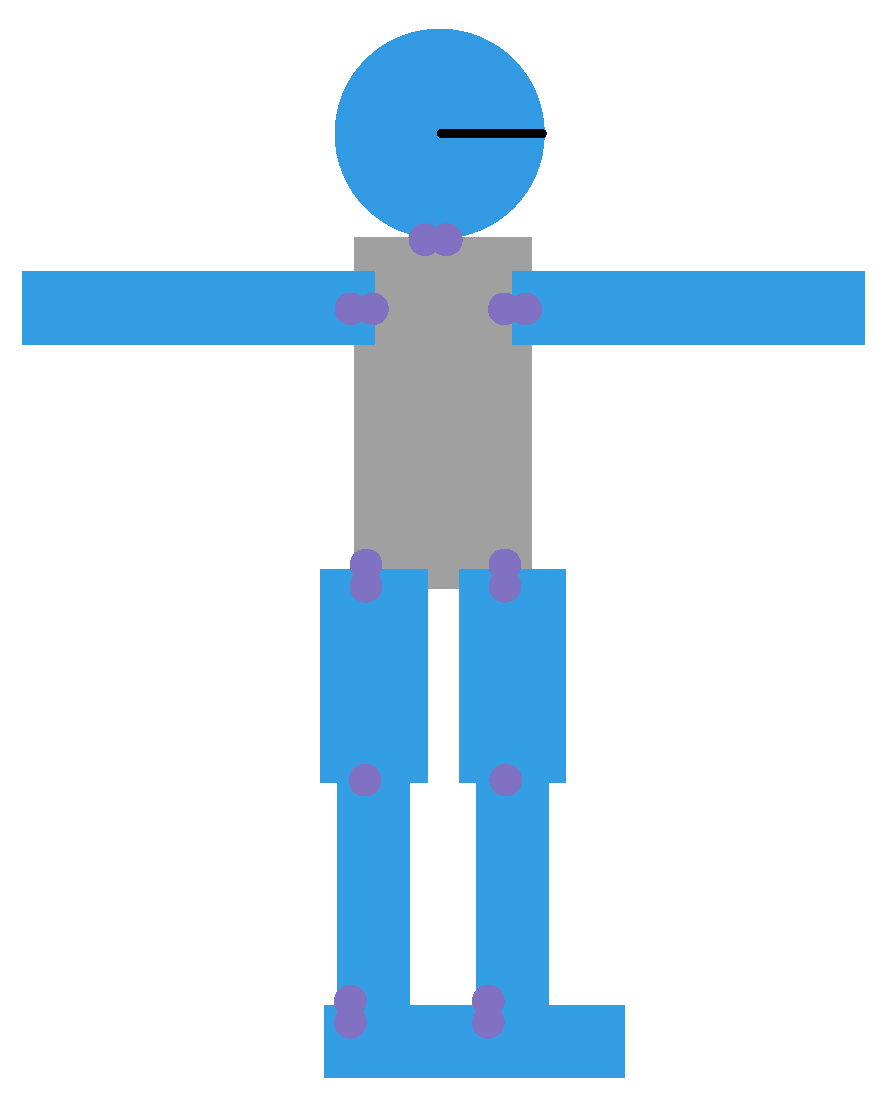
\includegraphics[scale=0.25]{humanoid-2d}
    \caption{Representation of 2D humanoid}
\end{figure}

The reward system developed for this environment:
\begin{itemize}
    \item Moves back: penalty of 200 points
    \item Stays in place: penalty of 100 points
    \item Moves forward: receives 0 points
    \item Both feet lose contact with the ground: cumulative penalty of 50 points
    \item Reaches target position: reward of 100 points
    \item Falls: penalty calculated as $\frac{1}{1-\gamma}\cdot$(highest penalty) 
\end{itemize}

\subsection{3D Walker}


\cite{ros-gym}


\chapter{Results}
    
\section{Cartpole Outcomes}
The first task developed was the classic cartpole environment,
this was helpfull in understanding core concepts of reinforcement learning and neural networks, along with it,
cartpole was essential in testing and setting up the logging interface as well as testing different implementations of the learning algorithm 
\subsection*{Keras-rl}
Keras-rl is a community maintained high level implementation of keras agents for reinforcement learning, this was the first implementaiton tested. 



The implementation of keras-rl is very easy and diesn't require a deep understanding of reinforcement learning and the leanring structure.
\subsection*{Keras API}
The second implementaiton tested was using the plain keras API, while this provides more flexibility it also requires a much deeper understandng of how reinforcement learning works.
%%%%%%%%% INSERT DETAILS HERE %%%%%%%%%
The implementaiton using the Keras API was essential to develop a necessary knowledge for the project and to progress to the next stage.
\subsection*{}

While an implementaiton using Keras-rl would be simpler and even possibly ease the itteration process, this implementation provides less flexibility and given the target of the project and 
desire to develop a deeper understanding of reinforcement learning the implementation using the Keras API was choosen to implemnt the next phases.

\subsection*{Results}

%%%%%%%%% INSERT RESULTS DATA AND ANALYSIS HERE %%%%%%%%%%%%%%%%%%

\section{2D Environment Outcomes}

\section{3D Environment Outcomes}

\section{Reward Function}



\chapter{Future Research}
    \section{Empowerment}

\section{Reward Function Development}

\section{Policy Gradients}

\section{Mujoco Implementation}

\section{Real Robot Training}


\chapter{Project Evaluation}
    \chapter{Project Evaluation}
Walking for bipedal robots using reinforcement learning was an ambitious project. Although walking could not be achieved, this project successfully developed a working 2D walking environment with a simple humanoid, implementing OpenAI Gym with ROS2 and developing documentation and preparation for future research on the topic.

The training for this project was mainly executed using Google colab+, as incompatibilities with the computer architecture (ARM64) made training locally slower in comparison. Although, Google colab constantly crashed due to timeouts and unknown problems, making it impossible to train for extended periods of time. 
On a retrospective, it would have been a better decision to train locally as even if the training was slower, it would be able to run for very long periods of time.

As already explored, the reward function should have been tested from the beginning exclusively with positive rewards, as this would have allowed for a more efficient experiment.



Although no training was executed, the last stage was a significant achievement as it is a useful tool and development not exclusive to this project but for the team. 

\chapter{Conclusion}
    \include{MainContent/conclusion.tex}
\bibliographystyle{plain}
\bibliography{reference}
\end{document}

